\documentclass[preprint,12pt]{elsarticle}

\biboptions{numbers,sort&compress}

\usepackage[margin=1in]{geometry}
\usepackage{amsmath,amssymb}
\usepackage{graphicx}
\usepackage{booktabs}
\usepackage{caption}
\usepackage[table]{xcolor}
\usepackage{url}
\captionsetup{font=small}

% Allow \texttt paths to break rather than run into the margin.
\renewcommand{\UrlFont}{\ttfamily}
\sloppy

\journal{bioRxiv preprint}

\begin{document}

\begin{frontmatter}

\title{A multi-channel iPSC-cardiomyocyte repolarization model does not beat a
hERG-only model on CiPA risk classification}

\author[perturb]{Daniel Reda\corref{cor1}}
\ead{daniel@perturb.bio}
\cortext[cor1]{Corresponding author. ORCID: 0000-0001-6160-6215.}
\affiliation[perturb]{organization={Perturb Bio, Inc.}, country={USA}}

\begin{abstract}
A multi-channel model of the human induced-pluripotent-stem-cell cardiomyocyte
(iPSC-CM) action potential must do more than a hERG-only model
before it can be adopted in a cardiotoxicity screen. We test one such model, the
Kernik-2019 iPSC-CM model run with a three-current Hill block, against that bar on two
endpoints and two measured datasets. On the three-class CiPA risk label the model scores
17 of 28 drugs, but that score is fragile: sweeping the supplied free exposure gives 16
of 28, with diltiazem the only change. A
hERG-only model, scored on the same 12/16 fit-and-freeze
split, scores 18 of 28 on the static hERG input and 19 of 28 on the dynamic input. The
hERG-only model scores higher. On the continuous repolarization readout the model does
better: against Blinova et al.\ (2018), with a Fridericia rate correction applied to
both sides, the model reaches a Spearman rank correlation of 0.70 over 112 matched
drug-dose points, against 0.62 for the hERG-only model, and its direction agreement on the
measurable points is 82 of 92 (89\%) against 72 of 92 (78\%) for both the hERG-only model and a
trivial always-prolong rule. Against Lee et al.\ (2025), the model recovers the measured
FPDc rank at 0.67 over the 75 non-quiescent drug-dose cells, but that correlation is
dose-dependent: 0.55 at $1\times$ $C_{\mathrm{max}}$ and 0.84 at $10\times$. Direction
agrees on 9 of 10 anchored drugs, against 6 of 10 for the hERG-only model. The added channels
capture the shortening direction of calcium-channel blockers, and they raise the rank
correlation. They do not improve the three-class risk label. We also report four negative or null results: the
population confidence signal is overconfident under both population models, adding
$I_{\mathrm{Ks}}$ is null, adding $I_{\mathrm{NaL}}$ degrades accuracy and moves nine
drugs, and the model's own mechanism recovery fails on most single-current and current-pair
tests.
The comparison against the hERG-only model, the full failure accounting, and the code and data are published
so the result can be reproduced.
\end{abstract}

\begin{keyword}
iPSC-cardiomyocyte \sep action potential \sep cardiotoxicity \sep validation \sep CiPA
\end{keyword}

\end{frontmatter}

\section{Introduction}\label{sec:intro}

In-silico models of the human ventricular action potential are proposed as an early
cardiotoxicity screen. A single strong current, the rapid delayed rectifier
$I_{\mathrm{Kr}}$ (hERG), dominates the QT-prolongation signal. A multi-channel model
therefore has to clear a specific bar: it must do more than a hERG-only model before it can be adopted in a safety package. This paper tests
that bar.

The model is the Kernik-2019 human iPSC-CM action-potential model \cite{kernik2019}.
It is an iPSC-CM model, the substrate CiPA recommends. We run it against two
independent measured datasets: Blinova et al.\ (2018) \cite{blinova2018}, the CiPA
multi-site myocyte validation study, and Lee et al.\ (2025) \cite{lee2025}, a 28-drug
iPSC-CM screen.

We ask two questions. First, on the three-class CiPA risk label, does the multi-channel
model beat a hERG-only model on the same fit-and-freeze split?
Second, on the continuous repolarization duration, does it reproduce the direction and
rank of the measured response better than the hERG-only model? The two answers differ, and that
difference is the finding.

\section{Methods}\label{sec:methods}

\paragraph{Model and solver}
The substrate is the Kernik-2019 iPSC-CM CellML model \cite{kernik2019}, run through
Myokit with the CVODE (SUNDIALS) adaptive solver. The model is autonomous: it carries
the Kernik $I_{\mathrm{f}}$ pacemaker current and no external stimulus, so it beats
spontaneously at about 61 beats per minute at baseline. Drug-free baseline values are
APD90 $= 413.31$~ms, MDP $= -75.60$~mV, cycle length $= 982.9$~ms, and rate
$= 61.0$~bpm.

\paragraph{Simulation protocol}
Every condition starts from the CellML initial state. We pre-pace for 10{,}000~ms to
settle the limit cycle, then log 8{,}000~ms at a 0.1~ms logging interval. An upstroke is
detected where $\mathrm{d}V/\mathrm{d}t$ crosses a fixed threshold. Cycle length is the mean
interval between successive peak-voltage times, and APD90 is the mean interval from
upstroke to 90\% repolarization over the detected beats. A condition with fewer
than two clean beats is recorded as missing. The 8{,}000~ms window is set so that even a
slow-beating, strongly blocked cell holds at least three upstrokes.

\paragraph{Drug block}
A compound is applied as fractional Hill block of the conductances
$g_{\mathrm{Kr}}$, $g_{\mathrm{CaL}}$, and $g_{\mathrm{Na}}$ (peak). The blocked fraction
at concentration $c$ is $1/(1+(c/\mathrm{IC50})^{h})$, with the reported $\mathrm{IC50}$
and Hill coefficient $h$. Exposures are the drug's free maximal concentration
($C_{\mathrm{max}}$) multiplied by 1, 2, 3, and 4. When a drug has no reference
$\mathrm{IC50}$ for a current, that current is not blocked. The hERG input is the static
Li-2017 fit distributed with the CiPA reference set (FDA/CiPA
\texttt{Li2017\_IC50.csv}, GPL-3.0); we also score a dynamic hERG column as a
cross-check. The $I_{\mathrm{CaL}}$ and $I_{\mathrm{Na}}$ (peak) inputs come from the
same reference set.

\paragraph{Risk label}
The risk score is the worst-case fractional APD90 prolongation across the 1--4$\times$
exposure grid. A cell that fails to repolarize is a collapse. The simulation marks a collapse
either by repolarization failure or by sustained depolarization above $-20$~mV for more than 50\%
of the trace. A collapse carries no duration, so it is recorded at a fixed ceiling of
twice the baseline prolongation. The ceiling is 826.6~ms of prolongation (an APD90 of
1{,}240~ms). It is a plotting convention and carries no predictive claim. Two cut points
on the
continuous score define the CiPA Low, Intermediate, and High classes. The cuts are fit on
the 12 training drugs and then frozen; the 16 validation drugs are scored blind.

\paragraph{Metrics}
We report the Spearman rank correlation between model APD90 prolongation and measured
FPD prolongation over three sets: all paired points, points with a completed
beat only, and points measurable on both sides (absolute response above 5~ms).
The 112 Blinova points are 28 drugs at four doses, and both variables rise
with dose inside a drug, so the pooled correlation counts each drug four times.
The pooled number is therefore inflated. We also report the per-dose correlation
(one value per drug, $n = 28$ at each dose) and the
per-drug correlation (one point per drug, from the mean over doses and the maximum
measured response). Direction agreement is the sign match between model and measurement.
We test it against a base rate: on the measurable set most points are positive, so
an always-prolong rule scores 72 of 92 (78\%), and we test the model's excess over that
base rate with a one-sided binomial test. Class balance is reported because the
operating point issues few or no Low calls.

\paragraph{Rate correction}
Blinova et al.\ and Lee et al.\ report Fridericia-corrected field potential duration
(FPDc). The model is a spontaneously-beating cell whose cycle length changes with drug,
so its uncorrected APD90 prolongation is not the quantity the measurement reports. We
apply the same correction to the model, $\mathrm{APD90c} = \mathrm{APD90}/(\mathrm{CL}_s)^{1/3}$
with cycle length in seconds, and recompute every Blinova statistic on the corrected
delta. We report both the uncorrected and the corrected rank, and the corrected value is
the primary result.

\paragraph{Data}
The Blinova et al.\ (2018) analysis uses the released per-well Excel file. The measured
response at each drug and dose is the median of the released per-well $\Delta\Delta$FPDc
across sites, cell types, and platforms, following the study's own multi-site
aggregation. The contributing record count is uneven: it ranges from 1 (bepridil at
4$\times$) to 81. The Lee et al.\ (2025) comparison uses the drug directions and FPDc
values stated in the main text. For the full panel it uses the FPDc heatmap in
Figure~3 of that paper. The supplement reports per-drug percentage change in FPD as
image-only tables (Tables S2 to S4), which we did not digitize. Figure~3 gives FPDc at
four $C_{\mathrm{max}}$ ratios ($0.1\times$, $1\times$, $10\times$, $100\times$). We
digitize the figure into a signed ordinal in $[-4,+4]$ (\path{lee_fig3_extract.py}) and
rank the model against it. The ordinal is coarse, so we report the tie count at each dose
and treat the high-dose cells with caution.

\section{Results}\label{sec:results}

\subsection{The hERG-only model comparison on the CiPA risk label}

The hERG-only model scores higher. Table~\ref{tab:benchmark} gives the fit-and-freeze result for
the multi-channel model and for a hERG-only model on the same
data, split, and protocol. The hERG-only model reaches 18 of 28 on the static hERG input and 19 of
28 on the dynamic input; the multi-channel model reaches 17 of 28. One compound separates
them on the static column, and two on the dynamic column.

\begin{table}[!ht]
\centering
\caption{CiPA three-class benchmark, 12 training drugs with cuts fit and frozen, 16
validation drugs scored blind. The hERG-only model blocks $g_{\mathrm{Kr}}$ alone, on
the static or the dynamic hERG $\mathrm{IC50}$ column. The multi-channel model adds
$g_{\mathrm{CaL}}$ and $g_{\mathrm{Na}}$ (peak). The hERG-only model is the bar the Introduction
sets.}
\label{tab:benchmark}
\begin{tabular}{l c c c c}
\toprule
Classifier & Train (12) & Blind (16) & All 28 & Fitted cuts (lo / hi) \\
\midrule
Multi-channel ($I_{\mathrm{Kr}}+I_{\mathrm{CaL}}+I_{\mathrm{Na}}$) & 8 & 9 & \textbf{17} & $-0.1044$ / $0.3491$ \\
hERG-only model, static & 8 & 10 & \textbf{18} & $-2.0342$ / $-0.5893$ \\
hERG-only model, dynamic & 8 & 11 & \textbf{19} & $-1.7312$ / $-0.6569$ \\
\bottomrule
\end{tabular}
\end{table}

The model's 17th correct call is fragile. The score of diltiazem, the only Low drug the
model calls correctly, sits at $-0.104$ against a low cut of $-0.1044$, a margin of
order $10^{-3}$, and that cut is itself fit on diltiazem's own score. A sensitivity sweep
over the supplied free $C_{\mathrm{max}}$ gives 16 of 28 at the nominal exposure, with
diltiazem the sole difference. We treat 16 as the operating figure.

The head-to-head on individual drugs does not favor the model. The model is right and
the hERG-only model is wrong on two drugs, astemizole and risperidone. The hERG-only model is right and the
model is wrong on three, loratadine, nifedipine, and nitrendipine. Verapamil is wrong for
both. Astemizole is the strongest single case for a multi-channel read: it was withdrawn
over QT prolongation, but its hERG IC50 (33.3~nM) is 128 times its free
$C_{\mathrm{max}}$ (0.26~nM), so the hERG-only model calls it Low while the model calls it
Intermediate, correctly. That one case does not offset the aggregate.

The operating point also has a class-balance defect. At the nominal exposure the model
issues 21 Intermediate calls and 7 High calls, and no Low calls at all. Nine drugs are
Low. In practice the three-class read is two-class, and it is wrong on every Low drug.

\subsection{The hERG-only model comparison on the continuous repolarization readout}

The result on the continuous readout is different. Against Blinova et al.\ (2018), with the
Fridericia correction applied to both sides, the multi-channel model reaches a Spearman
rank correlation of 0.70 over 112 matched points, against 0.62 for the static hERG-only model
and 0.57 for the dynamic hERG-only model. Excluding collapse points the model reaches 0.67,
against 0.54 for the hERG-only model. The model scores higher at every dose and on the
per-drug correlation (Table~\ref{tab:blinova}).

\begin{table}[!ht]
\centering
\caption{Blinova et al.\ (2018) rank agreement, multi-channel model against the
hERG-only model. Correlations are Spearman $\rho$. The pooled 112-point row is
pseudoreplicated (28 drugs $\times$ 4 doses); the per-dose rows ($n = 28$ each) and the
per-drug rows remove that dependence. ``Corrected'' applies the Fridericia correction to
the model APD90, matching the corrected FPDc the measurement reports.}
\label{tab:blinova}
\begin{tabular}{l c c c}
\toprule
Set & Multi-channel & hERG static & hERG dynamic \\
\midrule
All 112 points, uncorrected & 0.6714 & 0.6180 & 0.5728 \\
All 112 points, corrected & \textbf{0.7023} & 0.6179 & 0.5727 \\
Beat-only points, corrected & \textbf{0.6708} & 0.5437 & 0.5200 \\
Per-dose $1\times$, corrected & \textbf{0.7760} & 0.6873 & 0.6785 \\
Per-dose $2\times$, corrected & \textbf{0.8368} & 0.7398 & 0.6835 \\
Per-dose $3\times$, corrected & \textbf{0.7739} & 0.6652 & 0.6213 \\
Per-dose $4\times$, corrected & 0.5230 & 0.4136 & 0.2294 \\
Per-drug mean, corrected & \textbf{0.7593} & 0.6684 & 0.5233 \\
Per-drug maximum, corrected & \textbf{0.7838} & 0.7508 & 0.6237 \\
\bottomrule
\end{tabular}
\end{table}

\begin{figure}[!ht]
\centering
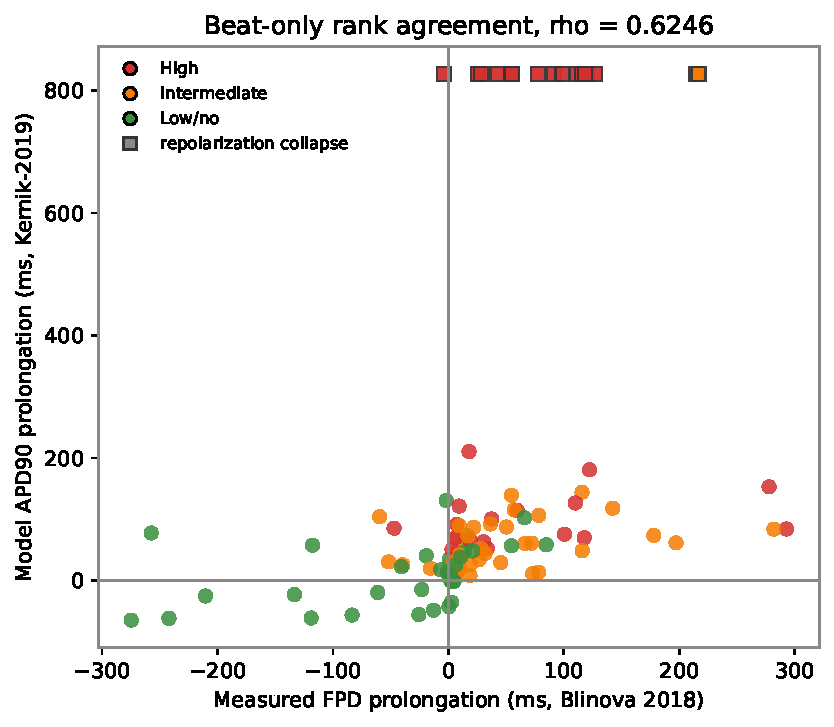
\includegraphics[width=0.72\textwidth]{figures/fig1_blinova_scatter.pdf}
\caption{Model APD90 prolongation against measured FPD prolongation, 112 matched
drug-dose points from Blinova et al.\ (2018). Colour is the CiPA TdP class. Squares are
model repolarization collapses, plotted at the fixed ceiling; their vertical position is
a convention, so the caption shows the beat-only correlation that excludes them. Values
here are uncorrected; the rate-corrected correlations are in Table~\ref{tab:blinova}.}
\label{fig:blinova}
\end{figure}

We compare direction agreement with a trivial always-prolong rule. On the points measurable
on the measured side, 92 of the 112, the model agrees with the measured sign on 82
(89\%). Both hERG-only models agree on 72 of 92 (78\%). That 78\% is the
always-prolong base rate: 72 of the 92 measurable medians are positive, and the hERG-only
model always prolongs. The model's 82 of 92 is 10 points above the base rate
(one-sided binomial $p = 0.0053$). The hERG-only model has no excess to report, because it cannot
go negative. The model produces a negative direction on only four drugs: diltiazem,
loratadine, nifedipine, and nitrendipine.

Direction agreement decays with dose. It is perfect at the clinical exposure and falls
across the grid: 18 of 18 at $1\times$, 22 of 23 at $2\times$, 23 of 26 at $3\times$, and
19 of 25 at $4\times$. The failure mode at high dose is the model over-prolonging. The
measured response saturates or reverses while the model keeps the block increasing.

\begin{figure}[!ht]
\centering
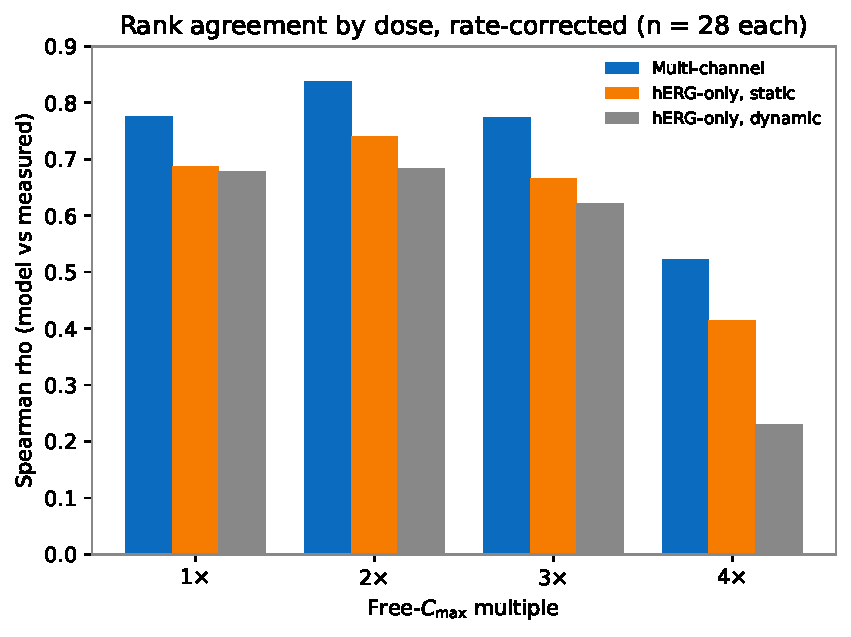
\includegraphics[width=0.72\textwidth]{figures/fig3_margin.pdf}
\caption{Rank agreement by free-$C_{\mathrm{max}}$ multiple, rate-corrected, for the
multi-channel model and the two hERG-only models. Each bar is a Spearman correlation
over the 28 drugs at that dose, so no drug is repeated within a bar. The multi-channel
model leads at every dose.}
\label{fig:margin}
\end{figure}

The 5~ms filter removes points whose measured response is small, so it is a measurement-side
filter. All 20 excluded points fail the
measured-side cut, and only 4 also fail the model-side cut. Direction agreement is 82\%
on all 112 points, 85\% under a model-side cut alone, and 89\% under the two-sided cut.
The filter also removes loratadine, the only drug in the panel for which Blinova
annotated no EAD. We report the two-sided figure as primary and the others as
sensitivity.

\subsection{The Lee et al.\ (2025) direction check}

Lee et al.\ measured FPDc across the same 28 CiPA drugs and published it as a signed
heatmap in Figure~3 of that paper. We digitize the heatmap into an ordinal and rank the
model against it. Pooled over the 75 non-quiescent drug-dose cells, the model ranks
against the measured FPDc at 0.67, the same value it reaches on the Blinova panel. The
pooled number hides a strong dose dependence. At $0.1\times$ and $1\times$
$C_{\mathrm{max}}$ the measured ordinals are coarse and mostly tied (27 of 28 values fall
in one bin at $0.1\times$), and the model ranks at 0.07 and 0.55. At $10\times$ the rank is
0.84 over 17 cells, and at $100\times$ it is 0.95 over only 4. One point per drug at its
maximum measured response gives 0.75 over 28 drugs. The model recovers the measured
ranking at supra-clinical exposure; at clinical exposure it only partly does.

\begin{table}[!ht]
\centering
\caption{Model against the Lee et al.\ (2025) FPDc heatmap at each $C_{\mathrm{max}}$
ratio. Rho is Spearman over the non-quiescent cells at that ratio. Direction is the sign
match; the model side uses a 5~ms deadband, the measured side is the sign of the ordinal.
Ties is the number of measured values that share a bin with another cell.}
\label{tab:leedose}
\begin{tabular}{c c c c c}
\toprule
$C_{\mathrm{max}}$ ratio & $n$ & Spearman $\rho$ & Direction & Tied measured cells \\
\midrule
$0.1\times$ & 28 & 0.07 & 11/28 & 27 \\
$1\times$ & 26 & 0.55 & 17/26 & 25 \\
$10\times$ & 17 & 0.84 & 16/17 & 17 \\
$100\times$ & 4 & 0.95 & 3/4 & 2 \\
\bottomrule
\end{tabular}
\end{table}

The per-dose ranks answer the question the Introduction sets. The model does not recover
the measured ranking at clinical exposure, and it does recover it as exposure rises.

We also keep a narrower direction check on ten anchored drugs (Table~\ref{tab:lee}), because
it isolates the calcium-blocker direction. The multi-channel model agrees on 9 of 10. The
hERG-only model agrees on 6 of 10. It cannot shorten, so it misses all four
calcium-channel blockers, nifedipine, nitrendipine, diltiazem, and verapamil. The
multi-channel model misses only verapamil.

\begin{table}[!ht]
\centering
\caption{Direction agreement on ten anchored drugs from Lee et al.\ (2025). TdP class is
the CiPA assignment. The multi-channel column is the model of this paper; the hERG
column is the hERG-only model.}
\label{tab:lee}
\begin{tabular}{l l c c c}
\toprule
Drug & TdP class & Lee measured & Multi-channel & hERG-only model \\
\midrule
quinidine & High & prolong & prolong & prolong \\
dofetilide & High & prolong & prolong & prolong \\
ibutilide & High & prolong & prolong & prolong \\
sotalol & High & prolong & prolong & prolong \\
droperidol & Intermediate & prolong & prolong & prolong \\
ranolazine & Low/no & prolong & prolong & prolong \\
nifedipine & Low/no & shorten & shorten & prolong \\
nitrendipine & Low/no & shorten & shorten & prolong \\
diltiazem & Low/no & shorten & shorten & prolong \\
verapamil & Low/no & shorten & \textbf{prolong} & prolong \\
\bottomrule
\end{tabular}
\end{table}

All eight of Lee's high-risk drugs prolonged FPDc by more than 20\% at the CiPA reference
doses, and the model prolongs all eight. Ranolazine also prolongs in both; at the
reference doses it is the only low/no-risk drug that Lee found to prolong FPDc past 20\%,
though at $10\times$ $C_{\mathrm{max}}$ mexiletine joins it. The calcium blockers
nifedipine, nitrendipine, and diltiazem shorten in both. The added channels are what
carry that shortening direction.

\subsection{Verapamil is the largest error in the dataset}

Verapamil is the single direction miss in the Lee check and it is the largest absolute
error in the Blinova comparison. In Blinova, measured $\Delta$FPDc at $2\times$, $3\times$,
and $4\times$ is $-19$, $-118$, and $-257$~ms. The model gives $+40$, $+58$, and
$+78$~ms. That is a 335~ms error at the top dose, and it is larger than the
error on any other drug. Verapamil is a calcium blocker whose hERG block is small, so the
model's hERG-dominated prolongation exceeds its calcium shortening. This is the known
calcium-block limitation of a hERG-weighted read, and it is the model's worst case. The
Lee check reproduces it, so two measured datasets show the error. The free-$C_{\mathrm{max}}$
sweep also moves verapamil, but that is a rerun of the model and not independent
evidence.

\subsection{The collapse flag carries almost no information}

The collapse flag looks better in raw counts than it is. The model collapses on six
drugs, and Blinova annotated an EAD for all six, so no collapse was a false positive. But
Blinova annotates an EAD somewhere for 27 of the 28 drugs, so the negative class holds a
single drug, loratadine. The full $2\times2$ is 6 collapse-with-EAD, 0
collapse-without-EAD, 21 no-collapse-with-EAD, and 1 no-collapse-without-EAD. A Fisher
exact test on that table gives $p = 1.0$. Drawing six drugs at random from a panel with
27 EAD drugs puts all six in the EAD class 79\% of the time. The claim that no collapse
was a false positive restates the base rate. Sensitivity is the only
informative count, and it is poor: the flag caught 6 of the 27 EAD-bearing drugs (22\%).

The collapse flag is more useful as a severity score than as a binary. Collapse severity,
the model's fractional prolongation short of the ceiling, ranks the measured EAD rate at
Spearman $\rho = 0.72$ ($p = 1.5\times10^{-5}$) and separates EAD-bearing from EAD-free
drugs at AUC 0.81. That is a stronger result than the binary flag and belongs in the
paper as a quantitative readout, with the caveat that the EAD-free class is a single
drug.

\section{Negative and null results}\label{sec:failure}

\paragraph{The population confidence signal is overconfident under both population models}
A population-of-models run (10 conductance draws, frozen cuts) assigns each drug a
confidence equal to the fraction of cells agreeing on the risk class. That confidence is
not calibrated (Fig.~\ref{fig:calib}). Under independent draws the point-biserial
correlation between confidence and correctness is $+0.17$ ($p \approx 0.38$ at
$n = 28$), and the top band reports a mean confidence of 0.99 while its accuracy is
0.63 ($n = 19$). Under correlated draws the correlation is $-0.06$, and the top band
(mean confidence 0.99, $n = 25$) has accuracy 0.56. We report both modes rather than
the positive one alone. The population argmax does not beat the deterministic call (0.57
against 0.61). The confidently-wrong drugs are the low-risk over-call set plus sotalol,
the same structural bias as the benchmark. We do not publish this confidence as a
probability.

\begin{figure}[!ht]
\centering
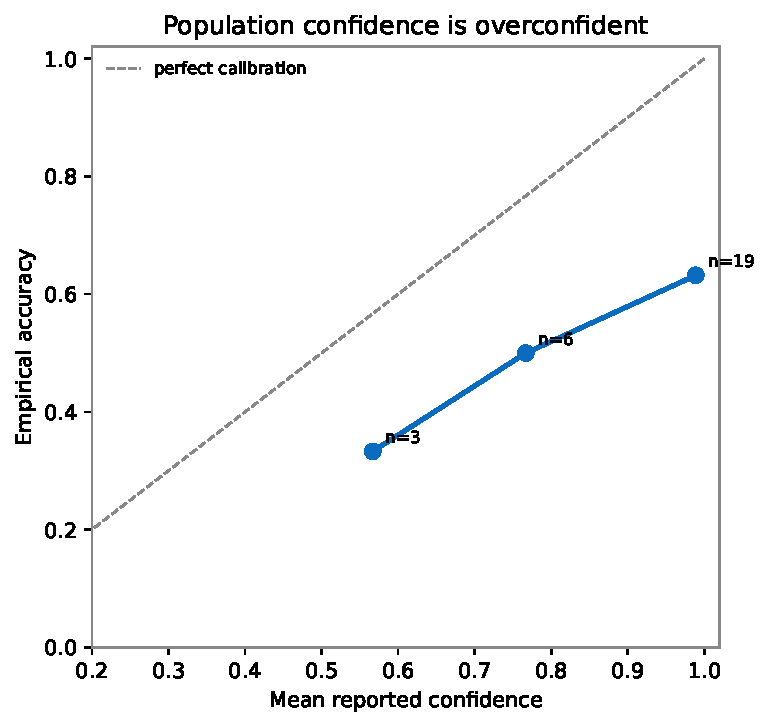
\includegraphics[width=0.72\textwidth]{figures/fig2_calibration.pdf}
\caption{Reliability bands for the population confidence signal, independent-draw mode.
Points fall below the identity line: reported confidence overstates achieved accuracy.
The correlated-draw mode is flatter still ($\rho = -0.06$) and is reported in the text.}
\label{fig:calib}
\end{figure}

\paragraph{Adding $I_{\mathrm{Ks}}$ is null}
Adding the slow delayed rectifier $I_{\mathrm{Ks}}$ to the risk score leaves the 28-drug
accuracy unchanged (17 of 28) and moves no drug's class; the largest movement is 0.001 in
fractional APD90. The result is null, but its scope is narrow: a reference
$I_{\mathrm{Ks}}$ $\mathrm{IC50}$ exists for only 7 of the 28 drugs, so the other 21 are
unchanged by construction. The reference $I_{\mathrm{Ks}}$ $\mathrm{IC50}$s block too
little at 1--4$\times$ free $C_{\mathrm{max}}$ to move this score. This is not a claim
that $I_{\mathrm{Ks}}$ is irrelevant to repolarization.

\paragraph{Adding $I_{\mathrm{NaL}}$ is negative, and the churn is large}
Adding an O'Hara-Rudy-style late sodium current lowers accuracy from 17 of 28 to 15 of
28, and from 9 of 16 to 7 of 16 on the blind split. The effect is not one correction. Nine
of the 28 classes change. Three move to their true class (mexiletine to Low, sotalol and
disopyramide to High), and six regress (verapamil to High and collapse, and cisapride,
clarithromycin, droperidol, pimozide, and terfenadine over-called High). High-risk false
positives go from 1 to 4. The cause is a shift in the baseline: at the pre-specified
conductance ($g_{\mathrm{NaL}} = 0.10$~mS/$\mu$F, a 1.03\% sustained late fraction) the
drug-free baseline APD90 lengthens from 413~ms to 588~ms. A 1\% persistent current should
not extend repolarization by 42\%, so either the conductance is large for this model or
the model holds thin repolarization reserve. The accuracy drop may follow from that
baseline shift rather than from the late current itself. The negative result is
therefore conditional on $g_{\mathrm{NaL}}$, not a property of $I_{\mathrm{NaL}}$ in
general.

\paragraph{The model's mechanism recovery fails}
A main use of the model is a mechanism ranking: which currents a compound blocks.
We tested whether the model recovers the true current profile from its own output, over
a grid of single-current and current-pair hypotheses. Single-current recovery
succeeds on 4 of 8 test cases. Pair recovery succeeds on 2 of 8, and the two successes
are both verapamil, the one drug whose pair the grid resolves. This is a self-test
against targets the same model generated, so it is not validation against wet data, but
it is a failure of the internal consistency the product depends on, and we report it
because we declare a competing interest in the model.

\paragraph{The exposure input is a first-class uncertainty}
The risk call hangs on the supplied free $C_{\mathrm{max}}$. Sweeping it over
0.5--2.0$\times$ with the cuts frozen leaves 17 of 28 calls stable and moves 11. High-risk
sensitivity rises from 4 of 8 to 7 of 8 across the range, and high-risk false positives
from 0 to 6. Six of the 11 flips are the model hitting the collapse ceiling. A read that
quotes a class without quoting the exposure it assumed is under-specified.

\section{Discussion}\label{sec:discussion}

The three-class CiPA risk label is decided against the multi-channel model. A hERG-only
model, fit and frozen on the same split, scores 18 of 28 on the static hERG input and 19
of 28 on the dynamic input, against 17 of 28 for the model of this paper. The label is a
threshold on a hERG-dominated risk, so a current that does not prolong the action
potential on its own rarely changes the class. Adding $I_{\mathrm{CaL}}$ and
$I_{\mathrm{Na}}$ block moves the repolarization duration without changing the class. On
this endpoint the extra channels add mechanism without adding accuracy.

The added channels improve the continuous readout. The multi-channel model reaches a rank
correlation of 0.70 against Blinova et al., against 0.62 for the hERG-only model, and it
agrees with the measured direction on 89\% of the measurable points against 78\%
($p = 0.005$). The hERG-only model cannot shorten, so it scores the always-prolong base
rate and misses every calcium-channel blocker. The multi-channel model recovers the
shortening, and that recovery is the source of its whole advantage. The channels do what
they were added to do, on the readout where their mechanism is visible.

The result sets the test for future claims. A multi-channel model offered as a better
classifier has to beat the hERG-only model on the three-class label, on the same split
and protocol. This model does not. A multi-channel model offered as a mechanistic or
continuous readout should be judged on that readout. Both claims can hold at once, and a
paper that reports only the second can appear stronger than it is. In short, the extra
channels improve the continuous readout. The regulatory risk class is unchanged.

\section{Limits of this validation}\label{sec:claims}

Established: the multi-channel model reproduces the rank and direction of measured
repolarization prolongation better than a hERG-only model. The added
channels carry the calcium-block shortening direction that the hERG-only model cannot produce.

Not established:
\begin{itemize}
\item Any advantage of the multi-channel model on the three-class CiPA risk
label, where the hERG-only model is equal or better.
\item Waveform or magnitude equivalence.
\item A rank correlation over the image-only supplement tables of Lee et al. We did not
digitize those values, so the full-panel rank we report rests on the coarse Figure~3 bins.
\item The mechanism ranking that is the main use, which has been tested only against
phenotypes the same model generated.
\end{itemize}

Four further limits apply. The model is a single deterministic myocyte, so a model
response is a point while a measured response is a distribution; the population run
addresses this only for the confidence signal. Both datasets are MEA field-potential
recordings, so neither tests the model against a patch-clamp action potential. The
Fridericia correction aligns the model and the measurement, but the model's APD90 and
the measured FPD remain different quantities. The 5~ms filter is defined on
the measurement and removes the one drug without a measured EAD.

\section*{Data and code}
The committed data, results, and analysis scripts are under \path{cipa_validation/}.
The Blinova comparison is produced by
\path{blinova_validation.py}, the comparison against the hERG-only model by \path{margin_comparison.py}, and
the rate correction by \path{rate_correction.py}. The Lee panel is digitized by
\path{lee_fig3_extract.py}, checked by \path{lee_fig3_verify.py}, and ranked by
\path{lee_comparison.py}. The calibration analysis is
\path{i2_calibration.py}; the $I_{\mathrm{Ks}}$, $I_{\mathrm{NaL}}$, collapse-severity,
and mechanism-recovery variants are \path{cipa_validation_harness_iks.py},
\path{cipa_validation_harness_inal.py}, \path{collapse_calibration.py}, and
\path{i1_mechanism_recovery.py}. The figures are regenerated from the committed result
files by \path{make_preprint_figures.py}. A versioned copy of the scripts and the result
files is available at \texttt{https://github.com/Perturb-Bio-Inc/cipa-validation} (tag
v1.0.0) and archived at OSF, DOI \texttt{10.17605/OSF.IO/JV4DZ}.

\section*{Declarations}
\paragraph{Funding} None.
\paragraph{Competing interests} The author is the sole founder of Perturb Bio, which
developed the in-silico read evaluated in this paper.

\begin{thebibliography}{99}
\bibitem{kernik2019}
D.C.~Kernik, S.~Morotti, H.~Wu, P.~Garg, H.J.~Duff, J.~Kurokawa, J.~Jalife,
J.C.~Wu, E.~Grandi, C.E.~Clancy.
\emph{A computational model of induced pluripotent stem-cell derived cardiomyocytes
incorporating experimental variability from multiple data sources}.
J.\ Physiol.\ 597(17):4533--4564, 2019. doi:10.1113/JP277724.

\bibitem{blinova2018}
K.~Blinova, Q.~Dang, D.~Millard, G.~Smith, J.~Pierson, L.~Guo, M.~Brock, H.-R.~Lu,
U.~Kraushaar, H.~Zeng, H.~Shi, X.~Zhang, K.~Sawada, T.~Osada, Y.~Kanda, Y.~Sekino,
L.~Pang, T.K.~Feaster, R.~Kettenhofen, N.~Stockbridge, D.G.~Strauss, G.~Gintant.
\emph{International multisite study of human-induced pluripotent stem cell-derived
cardiomyocytes for drug proarrhythmic potential assessment}.
Cell Rep.\ 24(13):3582--3592, 2018. doi:10.1016/j.celrep.2018.08.079.

\bibitem{lee2025}
S.-G.~Lee, M.W.~Kim, S.~Park, J.~Seok, J.~Kim, Y.~Kim, H.~Shin, Y.~Jeong,
J.H.~Park, M.~Lee, C.-Y.~Kim, H.M.~Chung.
\emph{Dual-cardiotoxicity evaluation of torsadogenic risk drugs using human
iPSC-derived cardiomyocytes}.
Biochem.\ Biophys.\ Res.\ Commun.\ 786:152756, 2025.
doi:10.1016/j.bbrc.2025.152756.
\end{thebibliography}

\end{document}
